%*============================================================*
%**Goal		:    文献分享:消失的女性与茶叶的价格
%**Author	:  	 ZhangYi zhangyiceee@163.com 15592606739
%**Created	:  	 20200323
%**Last Modified: 2020
%*============================================================*



\documentclass{beamer}
\usepackage[UTF8,noindent]{ctexcap}
\usepackage{natbib}
\usepackage{hyperref}


\graphicspath{{figures/}}




\usetheme{Madrid}
\usecolortheme{crane} %黄色
%Information to be included in the title page:
\title[文献分享:ZY]{消失的女性与茶叶价格--与特定性别有关的收入对性别失衡的影响}
\author[Nancy Qian 2008]{Nancy Qian	  2008}
\date{\today}

\begin{document}
\frame{\titlepage}
%开始你的表演



%第1页幻灯片
%==========================================
\begin{frame}
\frametitle{Abstract}
长期以来,经济学家一直争论发展中国家的性别失衡现象。本文利用后毛泽东时代的两项改革所带来的与特定性别有关的农业收入增长作为外生变量,来评估与特定性别相关的收入对存活孩子的性别比的影响。结果发现:在男性收入不变的前提下,女性收入提高增加了女孩的存活率;在女性收入不变的情况下,男性收入的增长则降低了女孩的存活率。
\\ 母亲收入的增加能提高所有孩子的受教育水平,父亲的收入增加则降低了女孩的受教育水平,但对男孩却没有影响。
\end{frame}


%第2页幻灯片
%==========================================
\begin{frame}
\frametitle{Problem \& Objective}
\begin{itemize}
 	\item 性别比例失衡是亚洲人口的一个特点,中国和印度表现尤为明显,阿马蒂亚·森称之为"失踪女性"
	\item 文章想研究女性相关工作的收入如何影响男孩女孩的相关产出,已有研究存在识别障碍:女性收入高的地区可能由于女性地位高。
	\item 作者希望通过后毛时代的两项改革来解决遗漏变量问题,进而识别因果效应。
\end{itemize}
毛泽东时代,中央计划生产指标以主粮作物为主(如小麦等),1978-1980年带的改革却提高了经济作物的回报(包括茶叶和果树),女性在采茶方面具有比较优势,男性在果树种植方面有比较优势,改革使得茶农家庭的总收入提高,女性的相对收入也增加了。果园类似
\end{frame}


%==========================================
\begin{frame}
\frametitle{Approach}
\centering{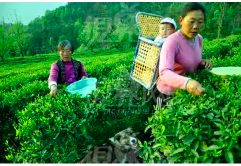
\includegraphics[scale=0.8]{women}}

\par 种植茶叶的县与不种植茶叶的县,改革使得茶叶的价值提高,比较改革前后这两类地区出生队列的性别比变化。
$$Diffenence-In-Difference$$

\end{frame}

%=========================================
\begin{frame}
\frametitle{Result}
在80年代初的中国农村
\begin{itemize}
	\item 在保持男性工资不变的情况下,提高成年女性收入10\%,女孩存活率提高1\%,男孩和女孩的受教育程度都提高了0.5年
	\item 相反,在保持女性收入不变情况下,男性收入的提高降低了女孩的存活率,降低了女孩的受教育程度,对男孩的受教育程度没影响。
\end{itemize}
\end{frame}

%==========================================
\begin{frame}
\frametitle{优势}
	\begin{itemize}
		\item 一系列混杂因素在这个时期的中国是固定的;
		\item 人口流动被严格控制;茶叶生产技术进步不大;性别选择技术在大部分农村地区不可用;
		\item 严格的计划生育政策在很大程度上控制了家庭规模
	\end{itemize}
	
\end{frame}

%==========================================

\begin{frame}
	\frametitle{Empirical Strategy}
用茶叶价值代表女性工资、果园的价值代表男性的工资,在中国茶叶主要由女性采摘(采茶要求心细),果园种植主要由男性负责(果树较高,对力量要求较高)由于1990年的人口普查数据无法直接用于研究性别专业化问题,因此使用农业部1993年全国固定点调查数据考察女性劳动力比例和茶叶播种之间的相关性。从表1中1-4列,每户家庭中茶叶播种量和茶叶耕地比例都与家庭中男性劳动力比例负相关。 
\\ 改革之前都是强制种植粮食,改革后,那些希望种植茶叶的家庭中:男性继续从事粮食生产,女性转向茶叶生产。此外,由于监督比较困难,因此雇佣工人的可能性比较低。

\end{frame}

\begin{frame}
\frametitle{表1}
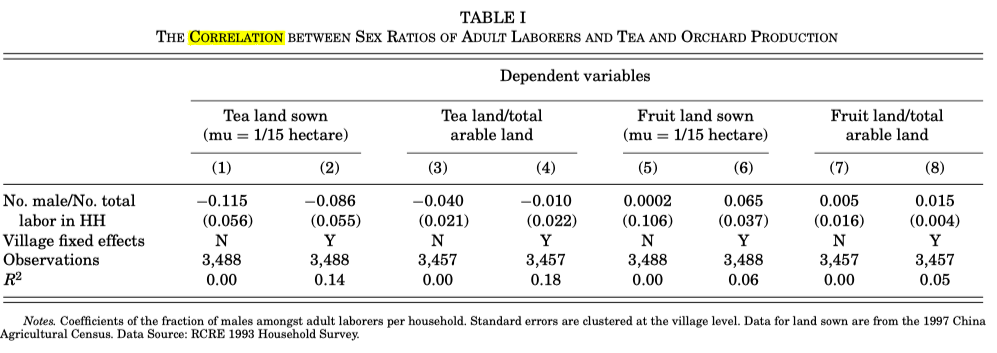
\includegraphics[scale=0.35]{table1}
\\ 1993年农村固定点观察数据,看家庭中男性劳动力比例与茶叶种植面积之间的相关性。
\end{frame}



%==========================================

%\begin{frame}
%	\centering
%	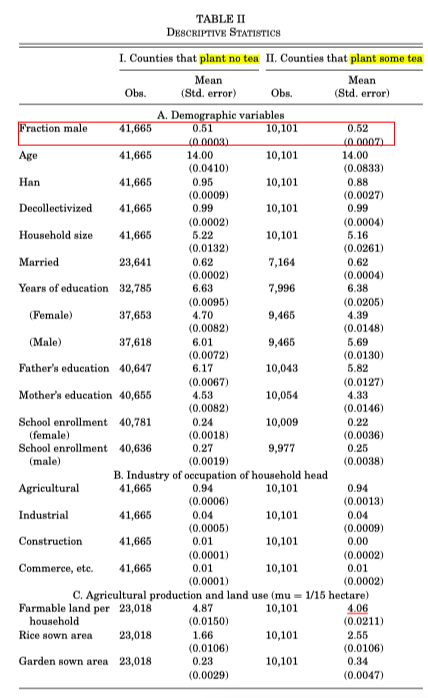
\includegraphics[scale=0.4]{table2}
%\end{frame}

%==========================================
\begin{frame}
\frametitle{政策背景}
    1978年之前,粮食生产严重集中,分配不公,缺乏贸易,农民缺乏积极性,采购价格被压低导致农村收入低,农作物被划为三类,前两种实施配额制
    \begin{enumerate} 
	\item 国民福利所必需的作物:谷物、所有油料作物和棉花
	\item 经济作物,包括果园产品和茶叶
	\item 其他农业项目
\end{enumerate}
\end{frame}

%==========================================
\begin{frame}
	\frametitle{政策背景}
1978年以后的改革(价格改革和家庭联产承包责任制)
\begin{enumerate}
	\item 1978年价格改革,农民生产积极性提高,主要农作物价格上升,但第二类作物的上升幅度大于第一类
	\item 1980年开始的家庭联产承保责任制(HPRS)
\end{enumerate}
两项政策促进了农业生产的多样化,提高了区域专业化程度,减少了粮食种植面积。

\end{frame}

%\begin{frame}
%        \frametitle{Figure 2}
%        \begin{columns}
%            \column{0.5\textwidth}
%            \begin{minipage}[c][0.4\textheight][c]{\linewidth}
%                \centering
%                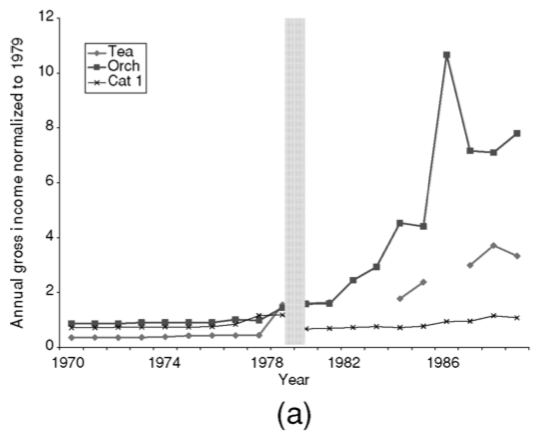
\includegraphics[width=0.8\linewidth]{figure2_a}
%            \end{minipage}
%
%            \begin{minipage}[c][0.4\textheight][c]{\linewidth}
%                \centering
%                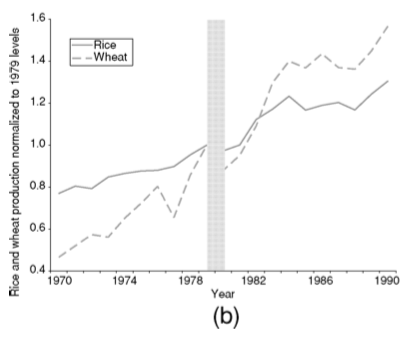
\includegraphics[width=0.8\linewidth]{figure2_b}
%            \end{minipage}
%            
%            \column{0.5\textwidth} % remember add this to the other clumn
%            \begin{minipage}[c][0.4\textheight][c]{\linewidth}
%               \centering
%                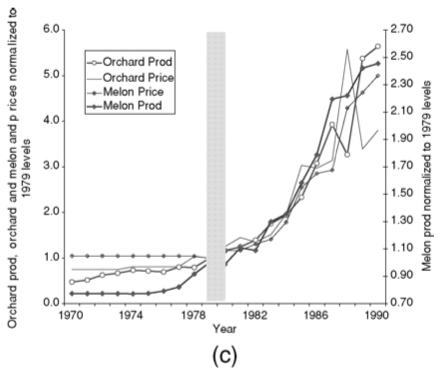
\includegraphics[width=0.8\linewidth]{figure2_c}
%            \end{minipage}
%
%            \begin{minipage}[c][0.4\textheight][c]{\linewidth}
%                \centering
%                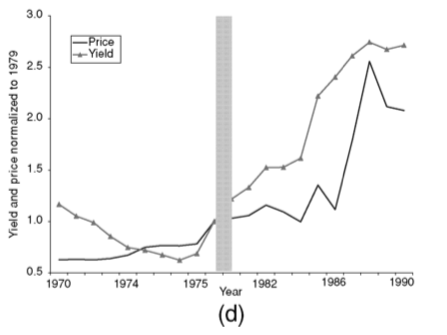
\includegraphics[width=0.8\linewidth]{figure2_d}
%            \end{minipage}
%        \end{columns}
%\end{frame}


\begin{frame}
\frametitle{Figure2}
	\begin{columns}
            \column{0.5\textwidth}
            \begin{minipage}[c][0.4\textheight][c]{\linewidth}
                \centering
                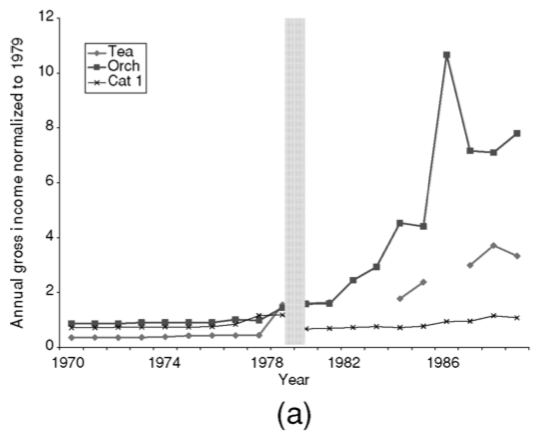
\includegraphics[width=0.8\linewidth]{figure2_a}
            \end{minipage}
            \begin{minipage}[c][0.4\textheight][c]{\linewidth}
                \centering
                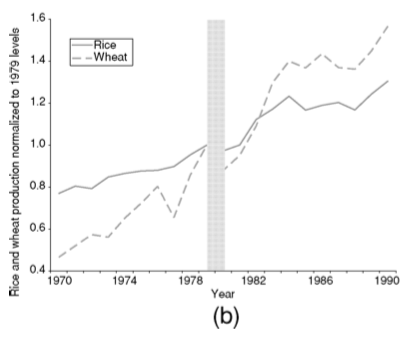
\includegraphics[width=0.8\linewidth]{figure2_b}
            \end{minipage}

            \column{0.5\textwidth} % remember add this to the other clumn
           	\begin{minipage}[c][0.4\textheight][c]{\linewidth}
            图a展示改革后种植茶叶和果园的带来的收入高于主粮作物,图b表示改革后第一类作物的产量不断增长,但增长速度没变(斜率没太大变化)
            \\ 注意这里的政策干预时点。
            \end{minipage}
    \end{columns}
\end{frame}


\begin{frame}
\frametitle{Figure2}
	\begin{columns}
            \column{0.5\textwidth}
            \begin{minipage}[c][0.4\textheight][c]{\linewidth}
                \centering
                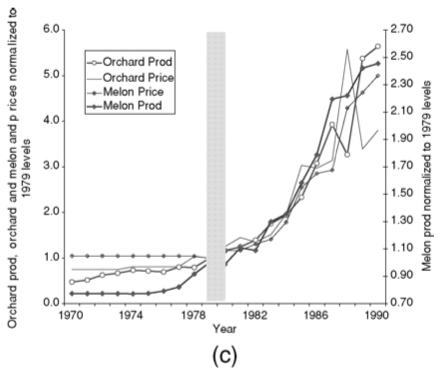
\includegraphics[width=0.8\linewidth]{figure2_c}
            \end{minipage}
            \begin{minipage}[c][0.4\textheight][c]{\linewidth}
                \centering
                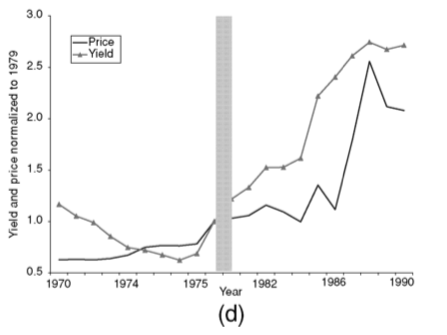
\includegraphics[width=0.8\linewidth]{figure2_d}
            \end{minipage}

            \column{0.5\textwidth} % remember add this to the other clumn
           	\begin{minipage}[c][0.4\textheight][c]{\linewidth}
            图c显示,瓜类和果园水果等第二类作物在改革后,随着采购价格的上涨,涨幅加快(陡峭)。在图d中可以看到茶叶也有类似的增长。
            \end{minipage}
    \end{columns}
\end{frame}

%==========================================
\begin{frame}
	\frametitle{Objective}
  与特定性别有关的收入对于性别失衡的影响
    \begin{itemize}
        \item 改革前后种植茶叶地区和未种植茶叶地区的男性比例变化
        \item 改革前后种植果园地区和未种植果园地区的男性比例变化
        \item 研究两类地区在改革前后男女受教育程度的变化
    \end{itemize}
\end{frame}


%==========================================
\begin{frame}
	\frametitle{识别策略}
识别策略是基于第二类作物的价格相对于第一类作物价格的提升,第一类作物的价格长期被压低,而第三类作物的价格一直未受到管制,因此第一类和三类作物价格变化对于改革前后男性比例无影响,检验的方程如下:
\begin{small}
\begin{equation}
    sex_{ic}=\sum_{l=1963}^{1990}(cat1_i*d_l)*\beta_l+\sum_{l=1963}^{1990}(cat3_i*d_l)\delta_l+Han_{ic}\zeta+\alpha+\psi_i+\gamma_c+\varepsilon_{ic}
\end{equation}
\end{small}
$sex_{ic}$是$i$县群组$c$的男性比例,其余以1962年为初始年份,具体结果见图3
同样
\end{frame}

%==========================================
\begin{frame}
	\frametitle{图3}
    \begin{columns}
            \column{0.6\textwidth}
            \begin{minipage}[c][0.4\textheight][c]{\linewidth}
                \centering
                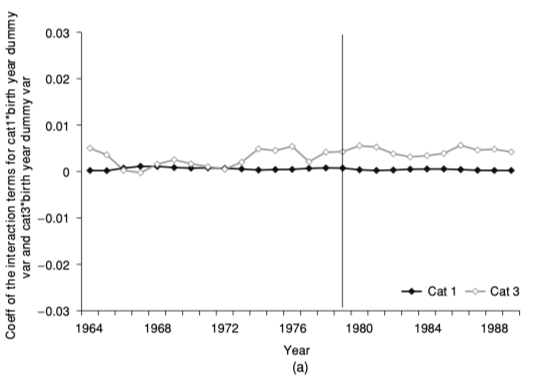
\includegraphics[width=0.8\linewidth]{figure3_a}
            \end{minipage}
            \column{0.4\textwidth} % remember add this to the other clumn
            \begin{minipage}[c][0.4\textheight][c]{\linewidth}
          性别比对于改革前后第一类和第三类作物价格变动产生的反应,可以看出第一类作物和第三类作物价格变动对于性别比的影响在改革前后的影响非常接近0。
            \end{minipage}
    \end{columns}
\end{frame}

\begin{frame}
    \frametitle{识别}
\begin{equation}
\begin{aligned}    
sex_{ic}=(tea_i*post_c)\beta+(orchard_i*post_c)\delta+ (cashcrop_i*post_t)\rho\\
+Han_{ic}\zeta +\alpha+\psi_i+\gamma_c+\varepsilon_{ic}
\end{aligned}
\end{equation}
$tea_i$指该地区种植茶叶的面积,如果茶叶价格上升,那么$\beta<0$ ,果园作物价格上升$\delta>0$

%,但是DID方法的一个缺陷是,它可能会将改革的影响与改革前或改革后可能发生的其他变化的影响混淆,那么DID估计出的结果就不会很好。
\end{frame}


%\begin{frame}
%  \frametitle{识别}
%  \begin{columns}
%            \column{0.6\textwidth}
%            \begin{minipage}[c][0.5\textheight][c]{\linewidth}
%                \centering
%                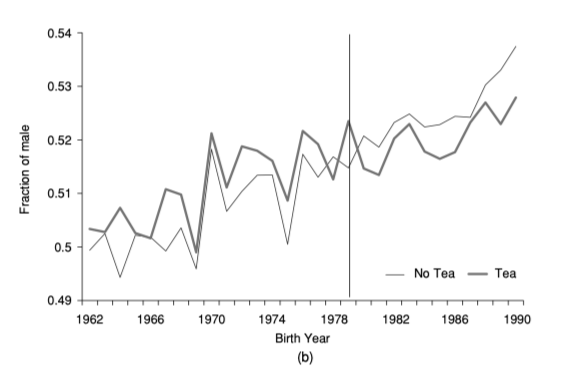
\includegraphics[width=0.9\linewidth]{figure3_b}
%            \end{minipage}
%            \column{0.4\textwidth} % remember add this to the other clumn
%            \begin{minipage}[c][0.4\textheight][c]{\linewidth}
%           茶叶种植区与非种植区的比较:茶叶种植区在改革前有更高的男性比例,改革后有更低的男%性比例,这说明本文的识别办法是可信的。
%            \end{minipage}
%    \end{columns}  
%\end{frame}


%================================


\begin{frame}
   \frametitle{识别IV} 
采用工具变量法,茶叶一般生长在温暖和半湿润的山顶上,避风避雨,采用每个县的平均坡度作为工具变量。
\\工具变量的第一阶段回归
\begin{equation}
    \begin{aligned}
         tea_i \times post_c=(slop_i \times post_c)\lambda+(cashcorp\times post_c)\phi+Han_{ic}\xi+ \\
        \alpha +\psi_{i}+post_c\eta+ \epsilon_{ic} 
    \end{aligned}
 \end{equation} 
 第二阶段回归
 \begin{equation}
    \begin{aligned}
sex_{ic}=(tea_i \times post_c)\beta +(cashcrop \times post_c)\phi +Han_ic \xi + \\ \alpha +\psi_{i}+post_c\eta+ \epsilon_{ic} 
    \end{aligned}
 \end{equation} 
\end{frame}

%\begin{frame}
%   \frametitle{概念框架} 
%性别选择技术在当时的年代并不常见,因此观察到的性别失衡可能是由于溺杀女婴等造成的,作者提出以%下四个可能通过茶叶价格提升而提高女婴存活率的路径:
%    \begin{itemize}
%        \item %可以通过增加父母对女儿的未来收入相对于儿子的收入的看法来增加生女孩的相对可取性
%        \item 女儿相对于儿子来说是奢侈品,那么家庭总收入的增加可以增加女孩的相对欲望
%        \item 增加女性特殊收入可以提高母亲的议价能力。如果母亲比父亲更喜欢女孩,这将提高女%性的相对存活率
%        \item 提高成年女性劳动力的价值,可以提高性别选择的成本,因为怀孕必须在孩子的性别显%示出来之前,就必须将孩子的性别进行到底
%    \end{itemize}
%    这里不赘述,具体可以看中文版中的分析。
%\end{frame}


%\begin{frame}
%    \frametitle{识别:IV}
%研究性别失衡的数据是1997年1\%农业普查的数据、1990年人口普查数据以及地理相关数据
%\\为了避免人口流动带来的混杂因素,因此作者将样本限制在同一个县居住5年以上的个体
%\\统计资料中低年龄阶段样本性别比存在不精确的情况,所以将样本限制在4岁及以上
%\\ 茶叶方面,并没有县一级茶叶的采购价格和产量的数据,因此作者使用1997年的农业普查的1\%样本%来代表1980年代初的农业状况,减少测量误差,但是这种情况下仍存在着测量误差。作者出于稳健性的考%量引入工具变量法。
%\end{frame}


\begin{frame}
    \frametitle{工具变量}
     \begin{columns}
            \column{0.5\textwidth}
            \begin{minipage}[c][0.4\textheight][c]{\linewidth}
                \centering
                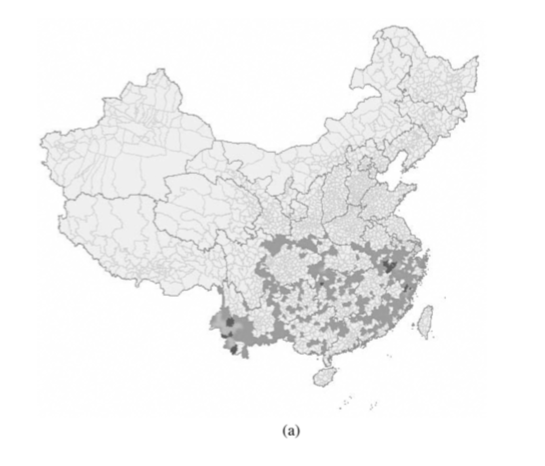
\includegraphics[scale=0.3]{figure4_a}
            图4—a 
            \\黑色地区为种植茶叶的地区
            \end{minipage}
          
            \column{0.5\textwidth} % remember add this to the 
            \begin{minipage}[c][0.4\textheight][c]{\linewidth}
                \centering
                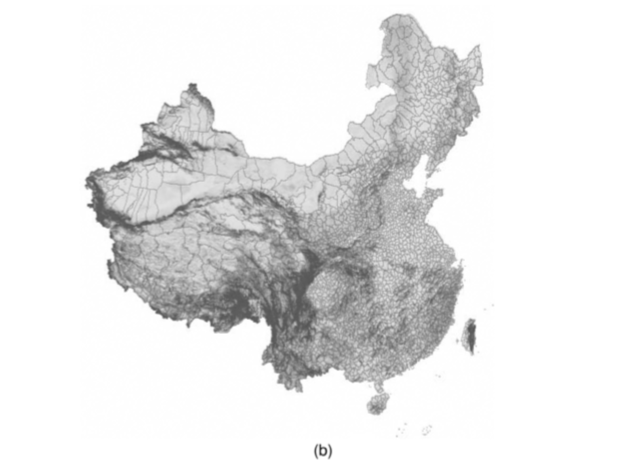
\includegraphics[scale=0.3]{figure4_b}
            图4-b
            \\黑色地区为比较陡峭的地区
            \end{minipage}
    \end{columns} 
\end{frame}

\begin{frame}
    \frametitle{Result}
  \begin{itemize}
        \item Result for survival rates
        \item Results on Educational Attainment
        \item Robustness
    \end{itemize}  
\end{frame}


\begin{frame}
    \frametitle{Result for survival rates}
    \begin{columns}
            \column{0.5\textwidth}
            \begin{minipage}[c][0.4\textheight][c]{\linewidth}
                \centering
                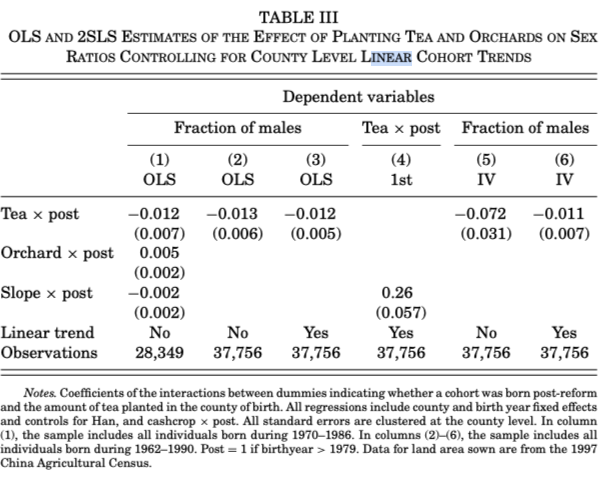
\includegraphics[scale=0.3]{table3}
             表3
            \end{minipage}
            \column{0.5\textwidth} % remember add this to the 
            \begin{minipage}[c][0.4\textheight][c]{\linewidth}
            表3的第一列(1970-1986年的样本)表示茶叶种植面积每增加一亩,男性的比例会降低1.2个百分点;果园种植面积每增加一亩,男性比例会提高0.5个百分点;种植普通作物对性别比无影响。
            \\  由于80年代的农业数据不可得,因此采用1997年的农业数据代表80年代的农业种植情况。
            \end{minipage}
    \end{columns} 
\end{frame}
\begin{frame}
   \frametitle{识别}
  算出每一年的影响大小
    \begin{equation}
    \begin{aligned}
sex_{ic}= \sum_{l=1963}^{1990}(tea_i*d_l)\beta_l+\sum_{l=1963}^{1990}(orchard_i*d_l)\delta_l+\sum_{l=1963}^{1990}(cashcrop_i*d_i)\rho_l\\
+Han_{ic}\zeta +\alpha+\psi_i+\gamma_c+\varepsilon_{ic}
    \end{aligned}
    \end{equation}
\end{frame}

\begin{frame}
    \frametitle{Result for survival rates}
    \begin{columns}
            \column{0.5\textwidth}
            \begin{minipage}[c][0.4\textheight][c]{\linewidth}
                \centering
                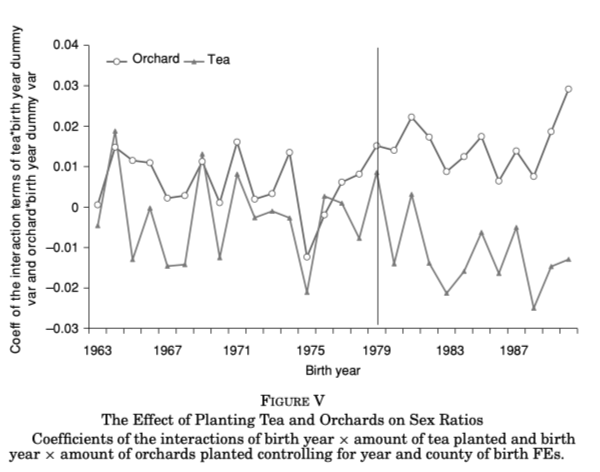
\includegraphics[scale=0.3]{figure5}
            图5
            \end{minipage}
            \column{0.5\textwidth} % remember add this to the 
            \begin{minipage}[c][0.4\textheight][c]{\linewidth}
            图5展示的是种植茶叶和果园地区价格变动在改革前后的对性别比的影响大小,可以认为性别比的变动是由于改革造成的。
            \end{minipage}
    \end{columns} 
\end{frame}


\begin{frame}
    \frametitle{Result for survival rates:IV}
为什么使用IV:1、由于使用的是1997年的农业数据来表征80年代初的农业情况,因此存在测量误差,可能会使得估计结果偏向0;2、OLS回归可能存在遗漏变量问题,(改革后偏好女孩的家庭种植茶叶)那么OLS估计量将高估茶叶价格上升对于性别比的影响。
            \\ 估计的效应=真实效应+性别偏好
\end{frame}


\begin{frame}
    \frametitle{Result for survival rates: IV }
     \begin{columns}
            \column{0.5\textwidth}
            \begin{minipage}[c][0.4\textheight][c]{\linewidth}
                \centering
                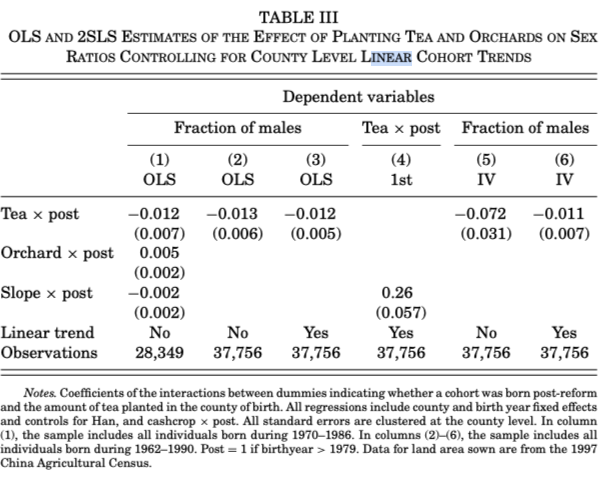
\includegraphics[scale=0.3]{table3}
                表3
            \end{minipage}
            \column{0.5\textwidth} % remember add this to the 
            \begin{minipage}[c][0.4\textheight][c]{\linewidth}
            表3的第4列展示的是工具变量的第一阶段回归,5、6列展示第二阶段回归,第6列展示的是控制了县级队列趋势后的估计值。尽管最后一列不显著了,但是与OLS的估计值几乎是相等的,这使得我们对于采用OLS方法得到的效应的文件性树立了信心。
            \end{minipage}
    \end{columns} 
\end{frame}



\begin{frame}
    \frametitle{Results on Educational Attainment}
    本分析采用2000年人口普查中0.05\%的县级出生年份数据,限定在已经完成教育的样本中,因此将样本限制在1962-1982年出生的人群中,参照对于性别比的影响,Y更换为受教育程度,分别看价格变动对于男女受教育程度的影响以及两者之间的差异。
\end{frame}

\begin{frame}
    \frametitle{Results on Educational Attainment}
    \centering{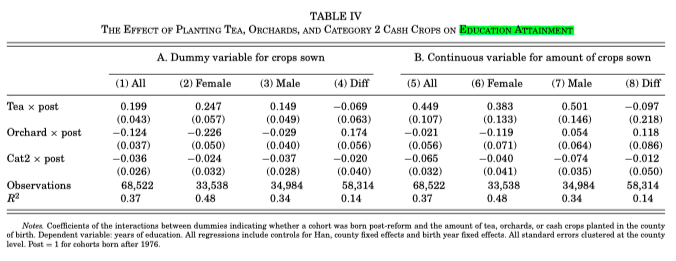
\includegraphics[scale=0.5]{table4}}
panel A 展示的是二值变量,B展示的是种植的连续变量回归结果,A显示提高茶叶种植面积能分别提高总体、男性和女性的受教育年限0.2、0.25和0.15年,但是果园种植却对于女性的受教育程度有负向影响(降低0.23年),对于男性没有影响
\\panel B 将X换为茶叶和果园的种植量,额外种植一亩的茶叶能提高女性(男性)受教育年限0.38年(0.5年),果园种植面积增加一亩,女性受教育程度降低0.12年,对男性无影响。
\end{frame}

\begin{frame}
    \frametitle{Results on Educational Attainment}
    \begin{columns}
            \column{0.5\textwidth}
            \begin{minipage}[c][0.4\textheight][c]{\linewidth}
                \centering
                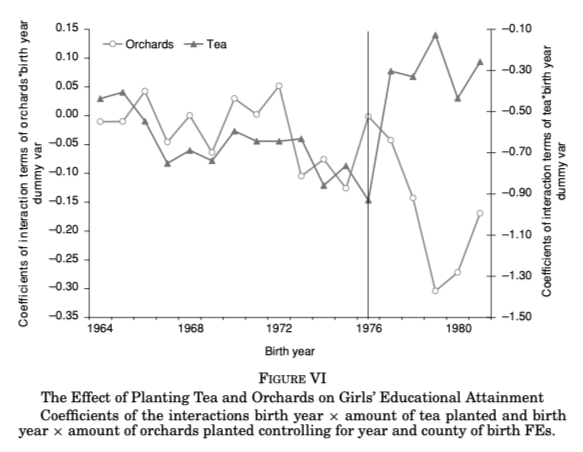
\includegraphics[scale=0.3]{figure6}
                图6
            \end{minipage}
            \column{0.5\textwidth} % remember add this to the 
            \begin{minipage}[c][0.4\textheight][c]{\linewidth}
            作者以1962年为基准年,在回归中纳入不同年份的虚拟变量,看系数的变化程度,可以看出在1976年以前,女性的受教育程度是在茶叶种植地区和果园种植地区是相似的,改革后果园地区的女性受教育程度降低,产茶地区的女性受教育程度增高了。
            \end{minipage}
    \end{columns} 
\end{frame}

\begin{frame}
    \frametitle{Robustness}
    \begin{itemize}
        \item Family Planning Policies
        \item Migration
    \end{itemize}
\end{frame}

\begin{frame}
    \frametitle{Robustness:family planning policies}
    计划生育:如果将计划生育政策的执行情况在种茶区和非种茶区之间进行系统的差异化,实证策略将混淆种茶与计划生育政策的效果。因此作者首先使用汉族和出生年份虚拟变量的交互项进行回归;第二、使用少数民族样本进行分析,结果依旧稳健。
\end{frame}


\begin{frame}
    \frametitle{Robustness:Migration}
    人口流动:如果人口流动在茶叶种植与未种植地区间存在差异,那么OLS的估计结果就是迁徙的影响而不是收入的效应,但是在研究所涉及的时间段内,农村地区的人口流动受到严格限制,所以迁移并不是一个重要的问题。
\end{frame}




\begin{frame}
    \frametitle{结论}
    无论是性别失衡还是教育投资,都会在短期内对与性别有关的收入做出变化。
\end{frame}

\begin{frame}
\frametitle{类似文献}
%\citet{Almond2019}研究土地改革对于性别选择的影响
 \citet{Adhvaryu2019}在加纳可可的价格决定了家庭的收入,将地区分两部分:种植可可(干预组,家庭收入受可可价格影响较大)和未种植可可的地区(对照组),研究母胎期间环境变化(可可价格的变动)对于成年后的影响,在早期生活中可可价格上升一个标准差,就会使出生在可可生产地区的群体在成年后出现严重精神痛苦的可能性比出生在未种植可可地区的群体降低3个百分点。

\end{frame}
\begin{frame}
    \frametitle{加纳}
    \centering
    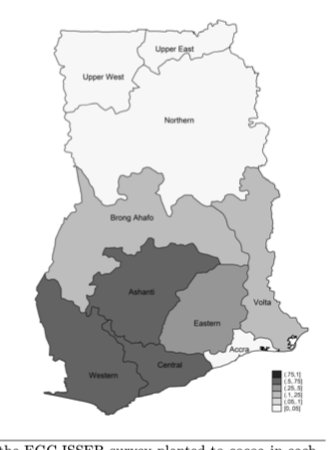
\includegraphics[scale=0.5]{ganna}
\end{frame}
\begin{frame}
    \frametitle{参考文献}
\bibliographystyle{plainnat}
\bibliography{references}
\end{frame}

%参考文献的案例 \citet{Krueger1999Experimental} \citep{Krueger1999Experimental}  注意两类的不同
\end{document}



